\subsection{Changes to the launcher}
\label{sub:changes_to_the_launcher}
In the current version of the launcher it is not possible to do anything without internet access, let alone use Week Schedule.
This is due to the process which takes place when the launcher is started. 
\begin{enumberate}
    \item Setup of the application; this includes graphics and the context
    \item\label{itm:sync} Fetch data from the remote server
    \item Prompt for login
    \item Show the home screen
\end{enumberate}
Since step~\ref{itm:sync} requires a connection to the remote server, the launcher halts if no such connection is available, hereby preventing any action or continuation.
While halted the launcher repeatedly tries to connect to the remote database, and will continue when said connection is established.
Moreover the current version of the GIRAF launcher will not allow reverting to step~\ref{itm:sync}, which implicates that once the fetching of data is done, one can only fetch data from the server again by forcing the launcher to terminate and restart.
This is far from optimal, since GIRAF is meant to replace any existing launcher on a given Android tablet, and forcing the launcher to restart in such a scenario would, for most users, mean restarting the tablet.
The long-term intent is for GIRAF to be usable regardless of whether a connection to the internet is available or not.
It is a wish of the customers that GIRAF works seamlessly whether an internet connection is available or not.
However, this user story only deals with the week schedule and making offline functionality for all other applications is therefore out of this user story's scope.
The seamlessness should also be present in a use case where a user loses internet for a short amount of time, which should not affect whatever task is being executed on the device. 

\bigskip \noindent
Making the launcher work without an internet connection causes certain problems in specific situations.
One such problem is when the launcher is started for the first time after installation or after the existing data has been erased --- i.e.\ simulating a clean installation. 
In this case the launcher and specifically its underlying local database contains no profiles to login with, thus preventing virtually any part of GIRAF to be used. 
The user should therefore be stopped and forced to obtain an internet connection in order to continue the use of GIRAF as operating the system without data is useless. 
The foundation of this complication lies in the organisational and administrative restrictions on GIRAF, primarily the launcher which encapsulates the local database used by a majority of the GIRAF apps.\todo{What organisational and administrative restrictions are these? Why is the problem caused by the launcer?}
GIRAF is designed to be used by institutions, hence creating user profiles is not possible from within GIRAF, but is instead intended to already be initialised when a given institution engages in workflow revolving around GIRAF --- In other words the creation of profiles and other initial administrative tasks will be done from a web-interface outside of GIRAF.
Schedules and pictograms are also stored in the local database, the latter of which is fetched from the remote server at the initial launch along side user profiles.

\subsubsection{Solutions and Design}
A solution which could enable offline mode in the launcher, would be to introduce a \textit{Check if offline, then prompt}--step, which requests the user to decide if GIRAF should be started even though a connection to the internet is not available.
This would notify the user that certain actions and workflows might not be available, and hereby prepare the user that the workflow may be different than they are used to.
Consequently the launcher should not prompt the user with obtrusive dialogs because no internet is available; instead the GIRAF launcher should attempt to proceed the start up phase as normal, this means that the user should only be prompted if a problem arise.

\bigskip \noindent
Taking the aforementioned issues and conflicts into account it is necessary to modify the launcher, such that using it without an internet connection is not an inconvenience and works seamlessly as wanted by the customers. 

We design the flow diagram in \myref{fig:launcher_offline_flow} to present the use case of starting the launcher with the new solution
Two decisions are added to make offline use possible when the local database is populated with usable profiles.
Firstly the launcher checks if any profiles are present in the local database, if there are any it continues to the login screen, if not it checks whether the tablet is offline. 
If the tablet is offline it will wait for an internet connection such that it can fetch the profiles, and continue to the loading screen afterwards.
We need to perform both checks since offline use of GIRAF is allowed, but impossible without locally stored user profiles; the user should be shown the prompt as seen on \myref{fig:offline_initstart} should this obstacle arise.\footnote{Currently there is a service for synchronisation of data from a tablet to the remote database, however, this feature is disabled because it is not implemented fully, and therefore it is not included in the workflow discussed in this guide. Furthermore the synchronisation of data is planned to be replaced along with a new database in later sprints.}

\begin{figure}[h]
    \centering
    \resizebox{1\textwidth}{!}{
\begin{tikzpicture}[auto]
    \node [cloud, align=center] (start) {Start};
    \node [block, below = of start] (setup) {Setup application};
    \node [decision, right = of setup] (network) {Is offline?};
    \node [decision, right = of network] (hasprofiles) {Has profiles?};
    \node [block, right = of hasprofiles] (download) {Download profiles};
    \node [block, above = of download] (stopuser) {Wait for network connection};
    \node [block, below = of download] (cont) {Continue to login screen};
    \node [draw=none, left = of cont] (network_) {};
    \node [preDefProc, above right = of cont] (home) {\nodepart{two}{Go to homescreen}};

    \draw [line] (start) -- (setup);
    \draw [line] (setup) -- (network);
    \draw [line] (network) -- node {yes} (hasprofiles);
    \draw [line] (network) |- node [above right] {no} (cont);
    \draw [line] (hasprofiles) -- node {yes} (cont);
    \draw [line] (hasprofiles) -- node {no} (stopuser);
    \draw [line] (stopuser) -- (download);
    \draw [line] (cont) -| (home);

\end{tikzpicture}                                   
}

    \caption{Flow diagram of how the GIRAF launcher behaves upon launch.}\label{fig:launcher_offline_flow}
\end{figure}

\subsubsection{Implementation of Internet Connection Check}
In order to implement the checks presented in \myref{fig:launcher_offline_flow}, a function which checks for an available internet connection is needed, as there is already a way to check if the database is empty.
To easily enable other parts of GIRAF to check if a connection to the internet is available, we implement the check in the \texttt{giraf-component} library.
This is also to encourage reuse of code as well as a unified way of determining connection status.
We use the Android API to determine if any network interface has a connection e.g. if a cellular connection is available or if the device is connected to a WiFi network.
However this does not provide any information about a connection to the internet, only that a LAN is available.
To perform this check we utilise a shell command called \texttt{ping} which tests the reachability of any host with a given IP address.
In our implementation as seen on line~\ref{lst:networkutil_ping} in \myref{lst:networkutil}, we ping the Google nameserver.
The Google nameserver is chosen because of its uptime, however pinging the service which GIRAF uses to synchronise would be ideal, because this is the only connection we care about.
Due to future architectural changes to GIRAF and especially the way it synchronises with the remote database, we choose to use the Google nameserver for now.
Moreover, if the launcher reaches the blocking state of \enquote{offline without a populated local database} we implement a check, which uses the aforementioned technique to find out if a connection has been established.
If a connection to the internet is made, the launcher is then forced to restart, thus initiating the startup process again to fetch data from the remote server.
%Should I talk about how? (Maybe irrelevant)

\begin{lstlisting}[float, floatplacement=h!, caption={The class from the \texttt{giraf-component} library where network utilities are implemented, such as the method used to check if a connection to the internet is available}, label={lst:networkutil}]
public abstract class NetworkUtilities {
    /**
     * Checks whether or not the device is connected to the internet
     *
     * @param thisActivity references the activity, used to get connectivity manager
     * @return true or false based on the connection status
     */
    public static boolean isNetworkAvailable(Activity thisActivity) {
        ConnectivityManager connectivityManager = (ConnectivityManager) thisActivity.getSystemService(Context.CONNECTIVITY_SERVICE);
        NetworkInfo activeNetworkInfo = connectivityManager.getActiveNetworkInfo();
        if (activeNetworkInfo != null && activeNetworkInfo.isConnected()) {
            Runtime runtime = Runtime.getRuntime();
            try {
                Process ipProcess = runtime.exec("/system/bin/ping -c 1 8.8.8.8");(*@\label{lst:networkutil_ping}@*)
                int     exitValue = ipProcess.waitFor();
                return (exitValue == 0);
            } catch (Exception e)  { e.printStackTrace(); }
        }
        return false;
    }
}
\end{lstlisting}

\subsubsection{Home Screen in Offline Mode}
Once the user continues to the home screen of the launcher, i.e. where the GIRAF apps can be launched, there should be some indication of which apps can be used in offline mode. 
As stated previously the intent for GIRAF is that all functionality should be available in offline mode, however as of now only some of the GIRAF apps will create no conflicts with an offline mode, like the Timer for instance. 
Furthermore the user story asks for Week Schedule specifically to be used in offline mode, therefore we deem it to be \enquote{out of the scope} of the resolution to this user story to make offline functionality for all parts of GIRAF.
To indicate which applications currently are available in offline mode, we make the disabled apps transparent alongside having a red cross, which the citizens use as a cancelled message in their current paper solutions at the institutions.
This is done such that users of GIRAF are still able to see all applications installed on the device, since merely removing the app icons may cause users to believe that some applications have been uninstalled.
Furthermore we redefine the way the app icons are sorted such that any disabled app will always be placed after the enabled apps --- in \myref{fig:launcher_screenshots} the online (\ref{fig:online_homescreen}) and offline mode (\ref{fig:offline_homescreen}) can be seen.
As well as avoiding confusion among users, this also helps toward the goal of offline mode being as convenient as possible.
On \myref{fig:offline_homescreen} the home screen of the launcher is presented in offline mode, and along side the indication that some apps are disabled, a notification is placed in the bottom of the screen, to remind the user that there is no connection to the internet.
When tapping a disabled application the user is prompted by a dialog to tell them that this app is unusable without internet, as seen on \myref{fig:offline_disabled}. 
As the citizens might not be able to read, the red cross across the applications should also be enough information for them to interpret that it is not available.
As previously stated the end goal is for all parts of GIRAF to be usable in offline mode, hence reducing the opacity and overlayed a red cross for certain applications is a temporary solution, as we are only working on the week schedule as the other applications are out of scope for this user story as previously mentioned in this chapter.
The way we implement how the disabled apps are shown on the home screen is by defining a constant list of package names, which should be usable in offline mode.
Another solution could be to let each app define for them selves if they have offline capabilities, however this would require updates to all apps of GIRAF, and we therefore deem it undesirable as having this information in one place makes it easier to edit especially for the next semester students.

Now that the GIRAF Launcher is able to launch applications without an internet connection, the next subsection will discuss possible solutions of conflict handling.

\begin{figure*}[h!]
    \centering
    \begin{subfigure}[t]{0.47\textwidth}
        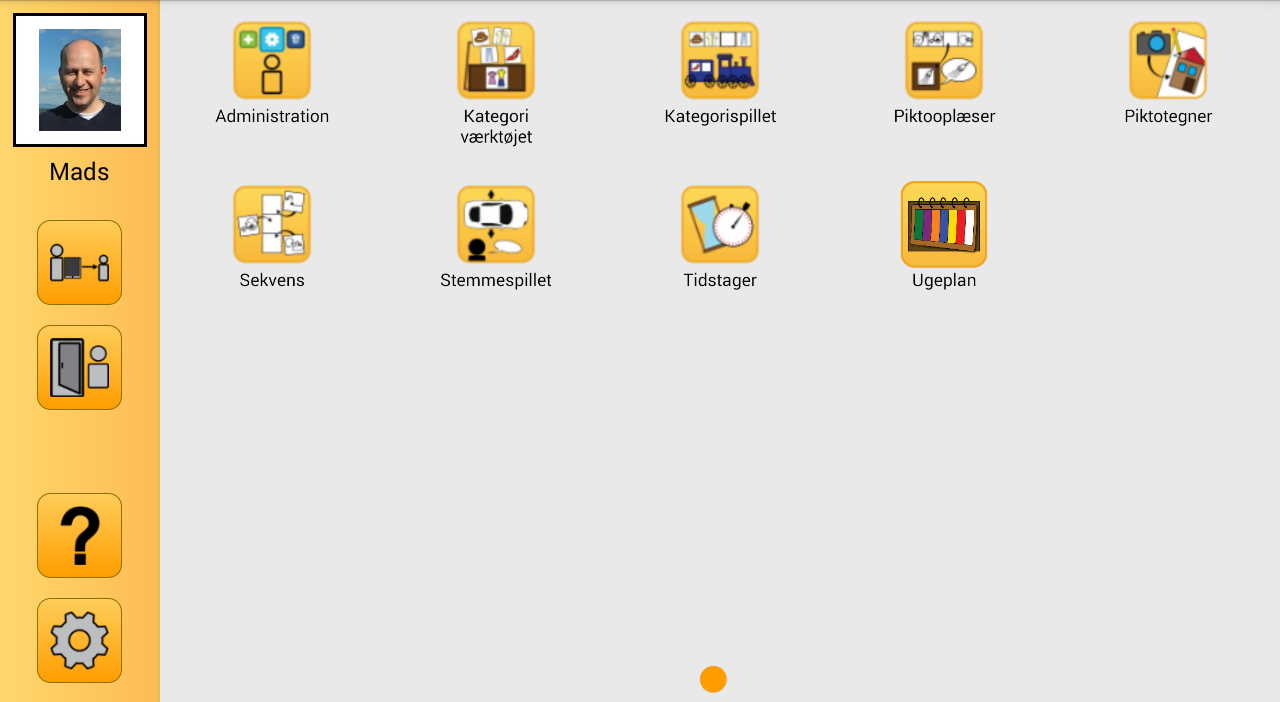
\includegraphics[width=\textwidth]{figures/img/screenshots/reg_homescreen.png}
        \caption{The home screen in online mode.}\label{fig:online_homescreen}
    \end{subfigure}%
    ~
    \begin{subfigure}[t]{0.47\textwidth}
        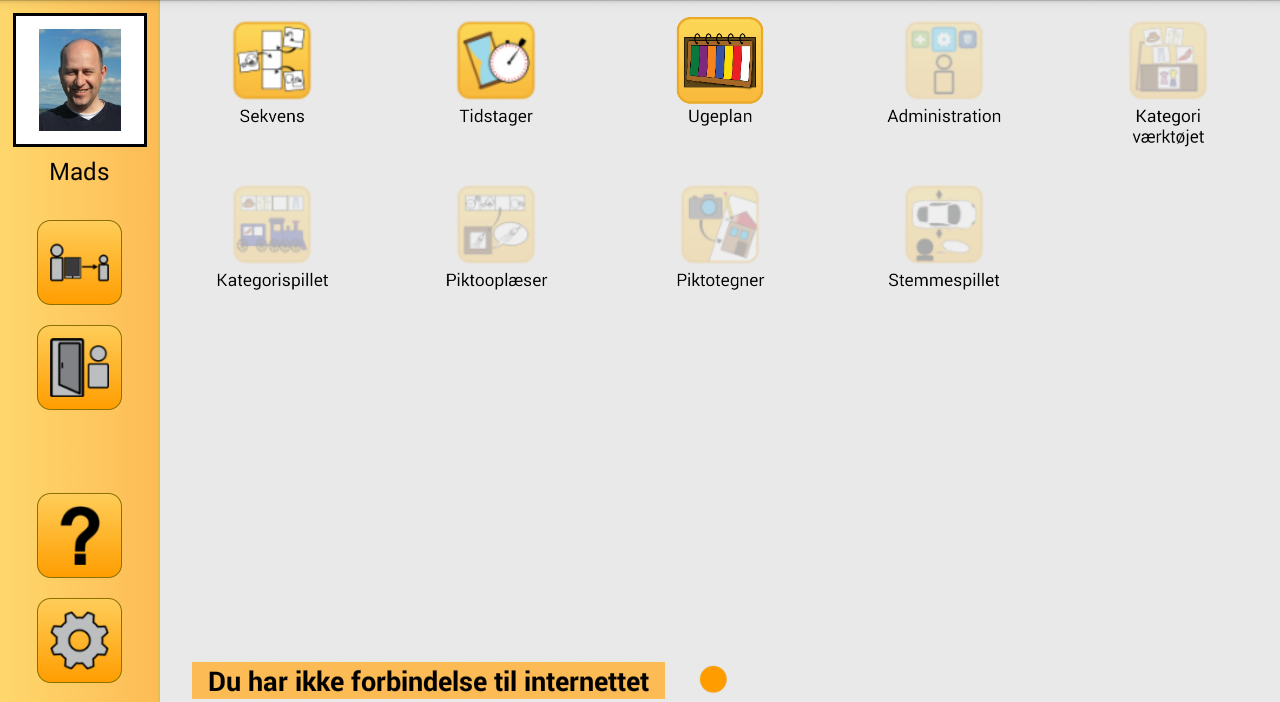
\includegraphics[width=\textwidth]{figures/img/screenshots/offline_homescreen.png}
        \caption{The home screen in offline mode.}\label{fig:offline_homescreen}
    \end{subfigure}
    \\
    \begin{subfigure}[t]{0.47\textwidth}
        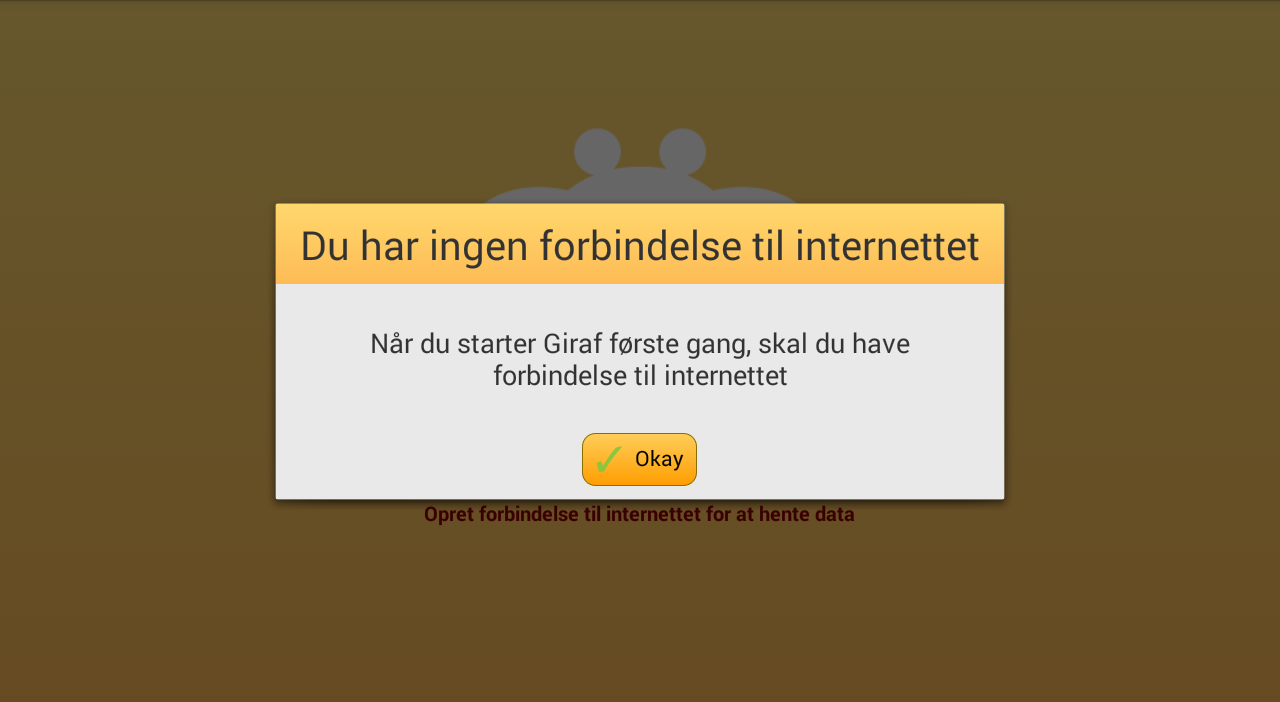
\includegraphics[width=\textwidth]{figures/img/screenshots/offline_initstart.png}
        \caption{Dialog which notifies the user that GIRAF must be started with an internet connection the first time.}\label{fig:offline_initstart}
    \end{subfigure}%
    ~
    \begin{subfigure}[t]{0.47\textwidth}
        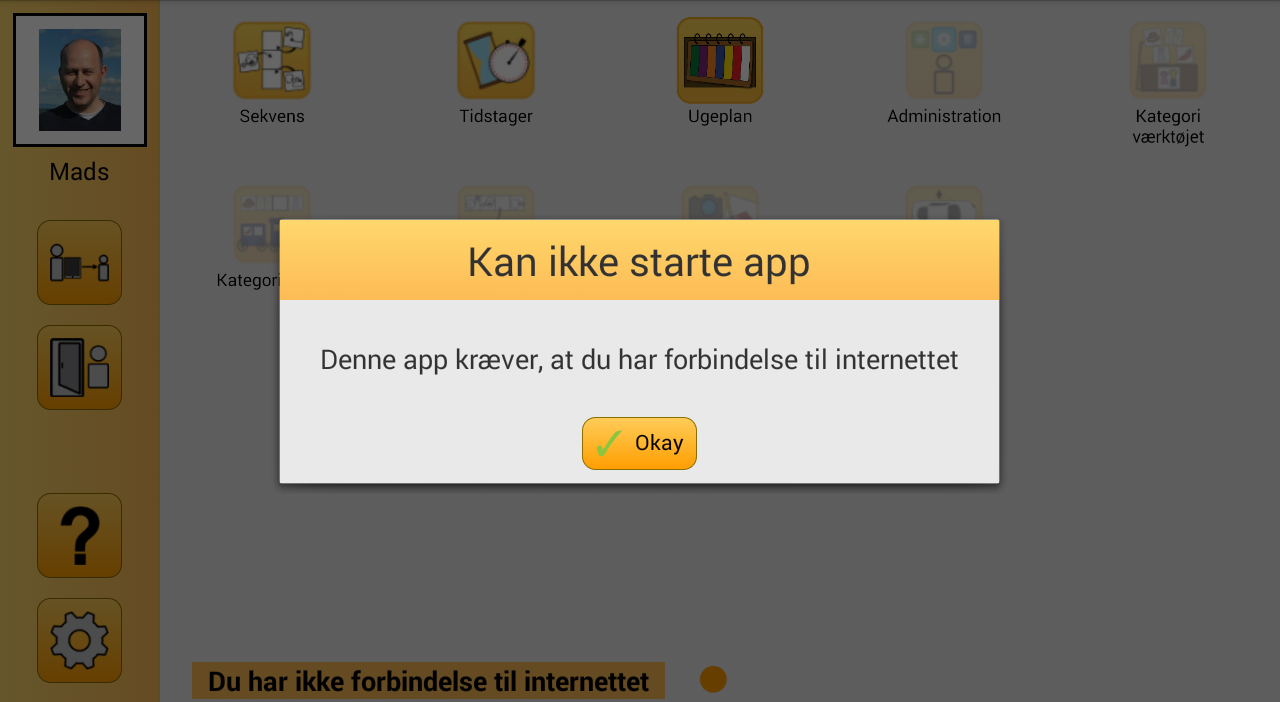
\includegraphics[width=\textwidth]{figures/img/screenshots/offline_disabled.png}
        \caption{Dialog which notifies the user that a given application cannot be used in offline mode.}\label{fig:offline_disabled}
    \end{subfigure}
    \caption{Screenshots from typical usage of the GIRAF launcher in both online and offline mode.}\label{fig:launcher_screenshots}
\end{figure*}\todo{Nye screenshots med krydserne henover istedet.}
    
